% Options for packages loaded elsewhere
\PassOptionsToPackage{unicode}{hyperref}
\PassOptionsToPackage{hyphens}{url}
%
\documentclass[
  12pt,
  a4paper,
  DIV=11,
  numbers=noendperiod]{scrreprt}

\usepackage{amsmath,amssymb}
\usepackage{setspace}
\usepackage{iftex}
\ifPDFTeX
  \usepackage[T1]{fontenc}
  \usepackage[utf8]{inputenc}
  \usepackage{textcomp} % provide euro and other symbols
\else % if luatex or xetex
  \usepackage{unicode-math}
  \defaultfontfeatures{Scale=MatchLowercase}
  \defaultfontfeatures[\rmfamily]{Ligatures=TeX,Scale=1}
\fi
\usepackage{lmodern}
\ifPDFTeX\else  
    % xetex/luatex font selection
\fi
% Use upquote if available, for straight quotes in verbatim environments
\IfFileExists{upquote.sty}{\usepackage{upquote}}{}
\IfFileExists{microtype.sty}{% use microtype if available
  \usepackage[]{microtype}
  \UseMicrotypeSet[protrusion]{basicmath} % disable protrusion for tt fonts
}{}
\usepackage{xcolor}
\usepackage{svg}
\setlength{\emergencystretch}{3em} % prevent overfull lines
\setcounter{secnumdepth}{5}
% Make \paragraph and \subparagraph free-standing
\ifx\paragraph\undefined\else
  \let\oldparagraph\paragraph
  \renewcommand{\paragraph}[1]{\oldparagraph{#1}\mbox{}}
\fi
\ifx\subparagraph\undefined\else
  \let\oldsubparagraph\subparagraph
  \renewcommand{\subparagraph}[1]{\oldsubparagraph{#1}\mbox{}}
\fi

\usepackage{color}
\usepackage{fancyvrb}
\newcommand{\VerbBar}{|}
\newcommand{\VERB}{\Verb[commandchars=\\\{\}]}
\DefineVerbatimEnvironment{Highlighting}{Verbatim}{commandchars=\\\{\}}
% Add ',fontsize=\small' for more characters per line
\usepackage{framed}
\definecolor{shadecolor}{RGB}{241,243,245}
\newenvironment{Shaded}{\begin{snugshade}}{\end{snugshade}}
\newcommand{\AlertTok}[1]{\textcolor[rgb]{0.68,0.00,0.00}{#1}}
\newcommand{\AnnotationTok}[1]{\textcolor[rgb]{0.37,0.37,0.37}{#1}}
\newcommand{\AttributeTok}[1]{\textcolor[rgb]{0.40,0.45,0.13}{#1}}
\newcommand{\BaseNTok}[1]{\textcolor[rgb]{0.68,0.00,0.00}{#1}}
\newcommand{\BuiltInTok}[1]{\textcolor[rgb]{0.00,0.23,0.31}{#1}}
\newcommand{\CharTok}[1]{\textcolor[rgb]{0.13,0.47,0.30}{#1}}
\newcommand{\CommentTok}[1]{\textcolor[rgb]{0.37,0.37,0.37}{#1}}
\newcommand{\CommentVarTok}[1]{\textcolor[rgb]{0.37,0.37,0.37}{\textit{#1}}}
\newcommand{\ConstantTok}[1]{\textcolor[rgb]{0.56,0.35,0.01}{#1}}
\newcommand{\ControlFlowTok}[1]{\textcolor[rgb]{0.00,0.23,0.31}{#1}}
\newcommand{\DataTypeTok}[1]{\textcolor[rgb]{0.68,0.00,0.00}{#1}}
\newcommand{\DecValTok}[1]{\textcolor[rgb]{0.68,0.00,0.00}{#1}}
\newcommand{\DocumentationTok}[1]{\textcolor[rgb]{0.37,0.37,0.37}{\textit{#1}}}
\newcommand{\ErrorTok}[1]{\textcolor[rgb]{0.68,0.00,0.00}{#1}}
\newcommand{\ExtensionTok}[1]{\textcolor[rgb]{0.00,0.23,0.31}{#1}}
\newcommand{\FloatTok}[1]{\textcolor[rgb]{0.68,0.00,0.00}{#1}}
\newcommand{\FunctionTok}[1]{\textcolor[rgb]{0.28,0.35,0.67}{#1}}
\newcommand{\ImportTok}[1]{\textcolor[rgb]{0.00,0.46,0.62}{#1}}
\newcommand{\InformationTok}[1]{\textcolor[rgb]{0.37,0.37,0.37}{#1}}
\newcommand{\KeywordTok}[1]{\textcolor[rgb]{0.00,0.23,0.31}{#1}}
\newcommand{\NormalTok}[1]{\textcolor[rgb]{0.00,0.23,0.31}{#1}}
\newcommand{\OperatorTok}[1]{\textcolor[rgb]{0.37,0.37,0.37}{#1}}
\newcommand{\OtherTok}[1]{\textcolor[rgb]{0.00,0.23,0.31}{#1}}
\newcommand{\PreprocessorTok}[1]{\textcolor[rgb]{0.68,0.00,0.00}{#1}}
\newcommand{\RegionMarkerTok}[1]{\textcolor[rgb]{0.00,0.23,0.31}{#1}}
\newcommand{\SpecialCharTok}[1]{\textcolor[rgb]{0.37,0.37,0.37}{#1}}
\newcommand{\SpecialStringTok}[1]{\textcolor[rgb]{0.13,0.47,0.30}{#1}}
\newcommand{\StringTok}[1]{\textcolor[rgb]{0.13,0.47,0.30}{#1}}
\newcommand{\VariableTok}[1]{\textcolor[rgb]{0.07,0.07,0.07}{#1}}
\newcommand{\VerbatimStringTok}[1]{\textcolor[rgb]{0.13,0.47,0.30}{#1}}
\newcommand{\WarningTok}[1]{\textcolor[rgb]{0.37,0.37,0.37}{\textit{#1}}}

\providecommand{\tightlist}{%
  \setlength{\itemsep}{0pt}\setlength{\parskip}{0pt}}\usepackage{longtable,booktabs,array}
\usepackage{calc} % for calculating minipage widths
% Correct order of tables after \paragraph or \subparagraph
\usepackage{etoolbox}
\makeatletter
\patchcmd\longtable{\par}{\if@noskipsec\mbox{}\fi\par}{}{}
\makeatother
% Allow footnotes in longtable head/foot
\IfFileExists{footnotehyper.sty}{\usepackage{footnotehyper}}{\usepackage{footnote}}
\makesavenoteenv{longtable}
\usepackage{graphicx}
\makeatletter
\def\maxwidth{\ifdim\Gin@nat@width>\linewidth\linewidth\else\Gin@nat@width\fi}
\def\maxheight{\ifdim\Gin@nat@height>\textheight\textheight\else\Gin@nat@height\fi}
\makeatother
% Scale images if necessary, so that they will not overflow the page
% margins by default, and it is still possible to overwrite the defaults
% using explicit options in \includegraphics[width, height, ...]{}
\setkeys{Gin}{width=\maxwidth,height=\maxheight,keepaspectratio}
% Set default figure placement to htbp
\makeatletter
\def\fps@figure{htbp}
\makeatother

\usepackage{indentfirst}
\usepackage{float}
\floatplacement{figure}{H}
\IfFileExists{plex-otf.sty}{
  %% Full TeXlive
  \usepackage[
    % math,
    RM={Scale=0.94},SS={Scale=0.94},SScon={Scale=0.94},TT={Scale=MatchLowercase,FakeStretch=0.9},
    DefaultFeatures={Ligatures=Common}
  ]{plex-otf}
  % \usepackage[Scale=MatchUppercase]{juliamono}
}{
  %% TinyTeX
  \usepackage{libertine}
}
\KOMAoption{captions}{tableheading}
\makeatletter
\@ifpackageloaded{caption}{}{\usepackage{caption}}
\AtBeginDocument{%
\ifdefined\contentsname
  \renewcommand*\contentsname{Содержание}
\else
  \newcommand\contentsname{Содержание}
\fi
\ifdefined\listfigurename
  \renewcommand*\listfigurename{Список иллюстраций}
\else
  \newcommand\listfigurename{Список иллюстраций}
\fi
\ifdefined\listtablename
  \renewcommand*\listtablename{Список таблиц}
\else
  \newcommand\listtablename{Список таблиц}
\fi
\ifdefined\figurename
  \renewcommand*\figurename{Рисунок}
\else
  \newcommand\figurename{Рисунок}
\fi
\ifdefined\tablename
  \renewcommand*\tablename{Таблица}
\else
  \newcommand\tablename{Таблица}
\fi
}
\@ifpackageloaded{float}{}{\usepackage{float}}
\floatstyle{ruled}
\@ifundefined{c@chapter}{\newfloat{codelisting}{h}{lop}}{\newfloat{codelisting}{h}{lop}[chapter]}
\floatname{codelisting}{Список}
\newcommand*\listoflistings{\listof{codelisting}{Листинги}}
\makeatother
\makeatletter
\makeatother
\makeatletter
\@ifpackageloaded{caption}{}{\usepackage{caption}}
\@ifpackageloaded{subcaption}{}{\usepackage{subcaption}}
\makeatother
\ifLuaTeX
\usepackage[bidi=basic]{babel}
\else
\usepackage[bidi=default]{babel}
\fi
\babelprovide[main,import]{russian}
\babelprovide[import]{english}
% get rid of language-specific shorthands (see #6817):
\let\LanguageShortHands\languageshorthands
\def\languageshorthands#1{}
\ifLuaTeX
  \usepackage{selnolig}  % disable illegal ligatures
\fi
\usepackage[style=gost-numeric,backend=biber,langhook=extras,autolang=other*]{biblatex}
\addbibresource{bib/cite.bib}
\usepackage{csquotes}
\usepackage{bookmark}

\IfFileExists{xurl.sty}{\usepackage{xurl}}{} % add URL line breaks if available
\urlstyle{same} % disable monospaced font for URLs
\hypersetup{
  pdftitle={Отчёта по лабораторной работе 2},
  pdfauthor={Нджову Нелиа},
  pdflang={ru-RU},
  hidelinks,
  pdfcreator={LaTeX via pandoc}}

\title{Отчёта по лабораторной работе 2}
\usepackage{etoolbox}
\makeatletter
\providecommand{\subtitle}[1]{% add subtitle to \maketitle
  \apptocmd{\@title}{\par {\large #1 \par}}{}{}
}
\makeatother
\subtitle{Математическое моделирование}
\author{Нджову Нелиа}
\date{}

\begin{document}
\maketitle

\renewcommand*\contentsname{Содержание}
{
\setcounter{tocdepth}{1}
\tableofcontents
}
\listoffigures
\listoftables
\setstretch{1.5}
\chapter{Цель
работы}\label{ux446ux435ux43bux44c-ux440ux430ux431ux43eux442ux44b}

Целью данной лабораторной работы является математическое моделирование
задачи преследования браконьерской лодки катером береговой охраны и
определение оптимальной траектории движения катера для перехвата цели.

\chapter{Задание}\label{ux437ux430ux434ux430ux43dux438ux435}

\begin{enumerate}
\def\labelenumi{\arabic{enumi}.}
\item
  Провести аналогичные рассуждения и вывод дифференциальных уравнений,
  если скорость катера больше скорости лодки в n раз (значение n задайте
  самостоятельно)
\item
  Построить траекторию движения катера и лодки для двух случаев.
  (Задайте самостоятельно начальные значения)
\item
  Определить по графику точку пересечения катера и лодки.
\end{enumerate}

\chapter{Выполнение лабораторной
работы}\label{ux432ux44bux43fux43eux43bux43dux435ux43dux438ux435-ux43bux430ux431ux43eux440ux430ux442ux43eux440ux43dux43eux439-ux440ux430ux431ux43eux442ux44b}

\emph{Вариант 64}

На море в тумане катер береговой охраны преследует лодку браконьеров.
Через определенный промежуток времени туман рассеивается, и лодка
обнаруживается на расстоянии 18,3 км от катера. Затем лодка снова
скрывается в тумане и уходит прямолинейно в неизвестном направлении.
Известно, что скорость катера в 4,9 раза больше скорости браконьерской
лодки.

Принимаем за \(t_0\) = 0, \(x_(л0) = 0\)- место нахождения лодки
браконьеров в момент обнаружения, \(x_(k0) = k = 18.3\) - место
нахождения катера береговой охраны относительно лодки браконьеров в
момент обнаружения лодки

Введем полярные координаты. Считаем, что полюс - это точка обнаружения
лодки браконьеров \(x_(л0)\) (\(\theta = x_(л0) = 0\)), а полярная осьr
проходит через точку нахождения катера береговой охраны

Траектория катера должна быть такой, чтобы и катер, и лодка все время
были на одном расстоянии от полюса \(\theta\) , только в этом случае
траектория катера пересечется с траекторией лодки.

Поэтому для начала катер береговой охраны должен двигаться некоторое
время прямолинейно, пока не окажется на том же расстоянии от полюса, что
и лодка браконьеров. После этого катер береговой охраны должен двигаться
вокруг полюса удаляясь от него с той же скоростью, что и лодка
браконьеров.

Чтобы найти расстояниеx (расстояние после которого катер начнет
двигаться вокруг полюса), необходимо составить простое уравнение. Пусть
через времяt катер и лодка окажутся на одном расстоянииx от полюса. За
это время лодка пройдет x, а катер k-x(или k+x, а в зависимости от
начального положения катера относительно полюса). Время, за которое они
пройдут это расстояние, вычисляется как x/v или k-x/4.9v (во втором
случае x+k/4.9v). Так как время одно и то же, то эти величины одинаковы.
Тогда неизвестное расстояниеx можно найти из следующего уравнения:

\[
\dfrac{x}{v} = \dfrac{k-x}{5.1v} \text{ -- в первом случае}
\]

\[
\dfrac{x}{v} = \dfrac{k+x}{5.1v} \text{ -- во втором}
\]

Отсюда мы найдем два значения \(x_1 = \dfrac{18.3}{5.9}\) и
\(x_2 = \dfrac{18.3}{3.9}\), задачу будем решать для двух случаев.

После того, как катер береговой охраны окажется на одном расстоянии от
полюса, что и лодка, он должен сменить прямолинейную траекторию и начать
двигаться вокруг полюса удаляясь от него со скоростью лодки \(v\). Для
этого скорость катера раскладываем на две составляющие: \(v_{r}\) -
радиальная скорость и - \(v_{\tau}\) тангенциальная скорость. Радиальная
скорость - это скорость, с которой катер удаляется от полюса,
\(v_r = \dfrac{dr}{dt}\). Нам нужно, чтобы эта скорость была равна
скорости лодки, поэтому полагаем \(\dfrac{dr}{dt} = v\).

Тангенциальная скорость -- это линейная скорость вращения катера
относительно полюса. Она равна произведению угловой скорости
\(\dfrac{d \theta}{dt}\) на радиус \(r\), \(r \dfrac{d \theta}{dt}\).

Получаем:

\[v_{\tau} = \sqrt{4.9^2v^2-v^2} = \sqrt{23.01v^2-v^2} = \sqrt{23.01}v\]

Из чего можно вывести:

\[
r\dfrac{d \theta}{dt} = \sqrt{23.01}v
\]

Решение исходной задачи сводится к решению системы из двух
дифференциальных уравнений:

\[\begin{cases}
&\dfrac{dr}{dt} = v\\
&r\dfrac{d \theta}{dt} = \sqrt{23.01}v
\end{cases}\]

С начальными условиями для первого случая:

\[\begin{cases}
&{\theta}_0 = 0\\  \tag{1}
&r_0 = x_1
\end{cases}\]

Или для второго:

\[\begin{cases}
&{\theta}_0 = -\pi\\  \tag{2}
&r_0 = x_2
\end{cases}\]

Исключая из полученной системы производную по \(t\), можно перейти к
следующему уравнению:

\[
\dfrac{dr}{d \theta} = \dfrac{r}{\sqrt{23.01}}
\]

Начальные условия остаются прежними. Решив это уравнение, мы получим
траекторию движения катера в полярных координатах.

Найдем точку пересечения траектории катера и лодки. Для этого найдем
аналитическое решение дифференциального уравнения, задающего траекторию
движения катера.

Решение Дифференциального уравнения и задачи Коши:

\[
\ln{r}=\frac{\theta}{\sqrt{23.01}} + C
\]

\[
r = Ce^\frac{\theta}{\sqrt{23.01}}
\]

\[
r = \frac{18.3}{5.9} e^\frac{\theta}{\sqrt{25.01}} \text{ -- для случая (1)}
\]

\[
r = \frac{18.3}{3.9} e^\frac{\theta+\pi}{\sqrt{25.01}}  \text{ -- для случая (2)}
\]

\section{Построение
модели}\label{ux43fux43eux441ux442ux440ux43eux435ux43dux438ux435-ux43cux43eux434ux435ux43bux438}

С помощью языка программирования Julia построим модель для приведенной
выше системы дифференциальных уравнений.

\begin{Shaded}
\begin{Highlighting}[]
\ImportTok{using} \BuiltInTok{DrWatson}
\PreprocessorTok{@quickactivate} \StringTok{"project"}
\ImportTok{using} \BuiltInTok{DifferentialEquations}
\ImportTok{using} \BuiltInTok{Plots}
\FunctionTok{gr}\NormalTok{(fmt}\OperatorTok{=:}\NormalTok{png)}
\end{Highlighting}
\end{Shaded}

\begin{verbatim}
┌ Warning: DrWatson could not find find a project file by recursively checking given `dir` and its parents. Returning `nothing` instead.
│ (given dir: /home/nelianjovu)
└ @ DrWatson ~/.julia/packages/DrWatson/2QF5p/src/project_setup.jl:84
\end{verbatim}

\begin{verbatim}
Plots.GRBackend()
\end{verbatim}

расстояние от лодки до катера

\begin{Shaded}
\begin{Highlighting}[]
\NormalTok{k }\OperatorTok{=} \FloatTok{18.3}
\end{Highlighting}
\end{Shaded}

\begin{verbatim}
18.3
\end{verbatim}

вычисление x для двух случаев

\begin{Shaded}
\begin{Highlighting}[]
\NormalTok{x1 }\OperatorTok{=}\NormalTok{ k}\OperatorTok{/}\FloatTok{5.9}   \CommentTok{\# для первого случая}
\NormalTok{x2 }\OperatorTok{=}\NormalTok{ k}\OperatorTok{/}\FloatTok{3.9}   \CommentTok{\# для второго случая}

\NormalTok{fi }\OperatorTok{=} \ConstantTok{pi}\OperatorTok{/}\FloatTok{4}  \CommentTok{\# угол под которым двигается лодка}
\end{Highlighting}
\end{Shaded}

\begin{verbatim}
0.7853981633974483
\end{verbatim}

движение лодки браконьеров

\begin{Shaded}
\begin{Highlighting}[]
\FunctionTok{x\_lodka}\NormalTok{(t) }\OperatorTok{=} \FunctionTok{tan}\NormalTok{(fi) }\OperatorTok{*}\NormalTok{ t}
\end{Highlighting}
\end{Shaded}

\begin{verbatim}
x_lodka (generic function with 1 method)
\end{verbatim}

функция, описывающая движение катера береговой охраны (ДУ)

\begin{Shaded}
\begin{Highlighting}[]
\FunctionTok{f}\NormalTok{(r, p, t) }\OperatorTok{=}\NormalTok{ r }\OperatorTok{/} \FunctionTok{sqrt}\NormalTok{(}\FloatTok{23.01}\NormalTok{)   }\CommentTok{\# n²{-}1 = 4.9²{-}1 = 24.01{-}1 = 23.01}
\end{Highlighting}
\end{Shaded}

\begin{verbatim}
f (generic function with 1 method)
\end{verbatim}

постановка ДУ с ЗК для 1 случая

\begin{Shaded}
\begin{Highlighting}[]
\NormalTok{prob }\OperatorTok{=} \FunctionTok{ODEProblem}\NormalTok{(f, x1, (}\FloatTok{0.0}\NormalTok{, }\FloatTok{2}\NormalTok{pi))}
\NormalTok{sol }\OperatorTok{=} \FunctionTok{solve}\NormalTok{(prob, saveat}\OperatorTok{=}\FloatTok{0.01}\NormalTok{)  }\CommentTok{\# шаг для красивой линии}
\end{Highlighting}
\end{Shaded}

\begin{verbatim}
retcode: Success
Interpolation: 1st order linear
t: 630-element Vector{Float64}:
 0.0
 0.01
 0.02
 0.03
 0.04
 0.05
 0.060000000000000005
 0.06999999999999999
 0.08
 0.09
 0.09999999999999999
 0.11
 0.12
 ⋮
 6.18
 6.1899999999999995
 6.2
 6.21
 6.22
 6.2299999999999995
 6.24
 6.25
 6.26
 6.27
 6.28
 6.283185307179586
u: 630-element Vector{Float64}:
  3.101694915254237
  3.1081677352886805
  3.1146540632289863
  3.1211539272628945
  3.1276673556376138
  3.1341943766598233
  3.1407350186956706
  3.1472893101707733
  3.1538572795702176
  3.1604389554385595
  3.1670343663798244
  3.1736435410575066
  3.18026650819457
  ⋮
 11.249092522785213
 11.272567865602353
 11.296092198300668
 11.319665623114163
 11.343288242491525
 11.36696015909611
 11.390681475805955
 11.414452295713767
 11.438272722126936
 11.46214285856752
 11.486062808772262
 11.493692525253868
\end{verbatim}

постановка ДУ с ЗК для 2 случая

\begin{Shaded}
\begin{Highlighting}[]
\NormalTok{prob\_2 }\OperatorTok{=} \FunctionTok{ODEProblem}\NormalTok{(f, x2, (}\OperatorTok{{-}}\ConstantTok{pi}\NormalTok{, }\ConstantTok{pi}\NormalTok{))}
\NormalTok{sol\_2 }\OperatorTok{=} \FunctionTok{solve}\NormalTok{(prob\_2, saveat}\OperatorTok{=}\FloatTok{0.01}\NormalTok{)}
\end{Highlighting}
\end{Shaded}

\begin{verbatim}
retcode: Success
Interpolation: 1st order linear
t: 630-element Vector{Float64}:
 -3.141592653589793
 -3.1315926535897933
 -3.1215926535897935
 -3.1115926535897933
 -3.1015926535897935
 -3.0915926535897933
 -3.0815926535897935
 -3.0715926535897933
 -3.0615926535897935
 -3.0515926535897933
 -3.0415926535897935
 -3.0315926535897932
 -3.0215926535897935
  ⋮
  3.0384073464102066
  3.0484073464102064
  3.058407346410207
  3.068407346410207
  3.0784073464102066
  3.0884073464102064
  3.098407346410207
  3.108407346410207
  3.1184073464102067
  3.1284073464102065
  3.138407346410207
  3.141592653589793
u: 630-element Vector{Float64}:
  4.6923076923076925
  4.702099907231594
  4.711912557192569
  4.721745684833609
  4.731599332887671
  4.741473544177681
  4.751368361616526
  4.761283828207066
  4.771219987042123
  4.7811768813044875
  4.791154554266915
  4.801153049292126
  4.811172409832812
  ⋮
 17.017857919646517
 17.053371899806976
 17.088959992864563
 17.124622353481
 17.160359136642768
 17.196170497661114
 17.232056592172043
 17.268017576136323
 17.30405360583949
 17.340164837891827
 17.37635142922841
 17.387893820829174
\end{verbatim}

построим траекторию движения лодки

\begin{Shaded}
\begin{Highlighting}[]
\NormalTok{ugol }\OperatorTok{=}\NormalTok{ [fi for i }\KeywordTok{in} \FloatTok{0}\OperatorTok{:}\FloatTok{0.1}\OperatorTok{:}\FloatTok{15}\NormalTok{]}
\NormalTok{x\_lims }\OperatorTok{=}\NormalTok{ [}\FunctionTok{x\_lodka}\NormalTok{(i) for i }\KeywordTok{in} \FloatTok{0}\OperatorTok{:}\FloatTok{0.1}\OperatorTok{:}\FloatTok{15}\NormalTok{]}
\end{Highlighting}
\end{Shaded}

\begin{verbatim}
151-element Vector{Float64}:
  0.0
  0.09999999999999999
  0.19999999999999998
  0.29999999999999993
  0.39999999999999997
  0.49999999999999994
  0.5999999999999999
  0.6999999999999998
  0.7999999999999999
  0.8999999999999999
  0.9999999999999999
  1.0999999999999999
  1.1999999999999997
  ⋮
 13.899999999999999
 13.999999999999998
 14.099999999999998
 14.199999999999998
 14.299999999999999
 14.399999999999999
 14.499999999999998
 14.599999999999998
 14.699999999999998
 14.799999999999999
 14.899999999999999
 14.999999999999998
\end{verbatim}

точное решение ДУ, описывающего движение катера береговой охраны

\begin{Shaded}
\begin{Highlighting}[]
\FunctionTok{y}\NormalTok{(x) }\OperatorTok{=}\NormalTok{ (k }\OperatorTok{*} \FunctionTok{exp}\NormalTok{(x }\OperatorTok{/} \FunctionTok{sqrt}\NormalTok{(}\FloatTok{23.01}\NormalTok{))) }\OperatorTok{/} \FloatTok{5.9}
\end{Highlighting}
\end{Shaded}

\begin{verbatim}
y (generic function with 1 method)
\end{verbatim}

подставим в точное решение угол, под которым движется лодка браконьеров

\begin{Shaded}
\begin{Highlighting}[]
\NormalTok{y\_result }\OperatorTok{=} \FunctionTok{y}\NormalTok{(fi)}
\end{Highlighting}
\end{Shaded}

\begin{verbatim}
3.653479338227613
\end{verbatim}

точка пересечения лодки и катера для 1 случая

\begin{Shaded}
\begin{Highlighting}[]
\FunctionTok{println}\NormalTok{(}\StringTok{"Точка пересечения лодки и катера для 1 случая: "}\NormalTok{, y\_result)}
\end{Highlighting}
\end{Shaded}

\begin{verbatim}
Точка пересечения лодки и катера для 1 случая: 3.653479338227613
\end{verbatim}

точное решение ДУ, описывающего движение катера береговой охраны для 2
случая

\begin{Shaded}
\begin{Highlighting}[]
\FunctionTok{y2}\NormalTok{(x) }\OperatorTok{=}\NormalTok{ (k }\OperatorTok{*} \FunctionTok{exp}\NormalTok{((x }\OperatorTok{+} \ConstantTok{pi}\NormalTok{) }\OperatorTok{/} \FunctionTok{sqrt}\NormalTok{(}\FloatTok{23.01}\NormalTok{))) }\OperatorTok{/} \FloatTok{3.9}
\end{Highlighting}
\end{Shaded}

\begin{verbatim}
y2 (generic function with 1 method)
\end{verbatim}

подставим в точное решение угол, под которым движется лодка браконьеров

\begin{Shaded}
\begin{Highlighting}[]
\NormalTok{y2\_result }\OperatorTok{=} \FunctionTok{y2}\NormalTok{(fi)}
\end{Highlighting}
\end{Shaded}

\begin{verbatim}
10.639577202489235
\end{verbatim}

точка пересечения лодки и катера для 2 случая

\begin{Shaded}
\begin{Highlighting}[]
\FunctionTok{println}\NormalTok{(}\StringTok{"Точка пересечения лодки и катера для 2 случая: "}\NormalTok{, y2\_result)}
\end{Highlighting}
\end{Shaded}

\begin{verbatim}
Точка пересечения лодки и катера для 2 случая: 10.639577202489235
\end{verbatim}

отрисовка траектории движения катера (1 случай)

\begin{Shaded}
\begin{Highlighting}[]
\NormalTok{p1 }\OperatorTok{=} \FunctionTok{plot}\NormalTok{(sol.t, sol.u, proj}\OperatorTok{=:}\NormalTok{polar, lims}\OperatorTok{=}\NormalTok{(}\FloatTok{0}\NormalTok{, }\FloatTok{15}\NormalTok{),}
\NormalTok{          label}\OperatorTok{=}\StringTok{"Траектория движения катера (случай 1)"}\NormalTok{,}
\NormalTok{          linewidth}\OperatorTok{=}\FloatTok{2}\NormalTok{, color}\OperatorTok{=:}\NormalTok{blue)}
\FunctionTok{plot!}\NormalTok{(p1, ugol, x\_lims, proj}\OperatorTok{=:}\NormalTok{polar, lims}\OperatorTok{=}\NormalTok{(}\FloatTok{0}\NormalTok{, }\FloatTok{15}\NormalTok{),}
\NormalTok{      label}\OperatorTok{=}\StringTok{"Траектория движения лодки"}\NormalTok{,}
\NormalTok{      linewidth}\OperatorTok{=}\FloatTok{2}\NormalTok{, color}\OperatorTok{=:}\NormalTok{red)}
\FunctionTok{title!}\NormalTok{(p1, }\StringTok{"Траектория движения катера и лодки (случай 1)"}\NormalTok{)}
\end{Highlighting}
\end{Shaded}

\includesvg{mathmod-lab02-report (Нджову Нелиа)_files/figure-pdf/cell-17-output-1.svg}

отдельный график для 2 случая

\begin{Shaded}
\begin{Highlighting}[]
\NormalTok{p2 }\OperatorTok{=} \FunctionTok{plot}\NormalTok{(sol\_2.t, sol\_2.u, proj}\OperatorTok{=:}\NormalTok{polar, lims}\OperatorTok{=}\NormalTok{(}\FloatTok{0}\NormalTok{, }\FloatTok{15}\NormalTok{),}
\NormalTok{          label}\OperatorTok{=}\StringTok{"Траектория движения катера (случай 2)"}\NormalTok{,}
\NormalTok{          linewidth}\OperatorTok{=}\FloatTok{2}\NormalTok{, color}\OperatorTok{=:}\NormalTok{green)}
\FunctionTok{plot!}\NormalTok{(p2, ugol, x\_lims, proj}\OperatorTok{=:}\NormalTok{polar, lims}\OperatorTok{=}\NormalTok{(}\FloatTok{0}\NormalTok{, }\FloatTok{15}\NormalTok{),}
\NormalTok{      label}\OperatorTok{=}\StringTok{"Траектория движения лодки"}\NormalTok{,}
\NormalTok{      linewidth}\OperatorTok{=}\FloatTok{2}\NormalTok{, color}\OperatorTok{=:}\NormalTok{red)}
\FunctionTok{title!}\NormalTok{(p2, }\StringTok{"Траектория движения катера и лодки (случай 2)"}\NormalTok{)}
\end{Highlighting}
\end{Shaded}

\includesvg{mathmod-lab02-report (Нджову Нелиа)_files/figure-pdf/cell-18-output-1.svg}

показать оба графика

\begin{Shaded}
\begin{Highlighting}[]
\FunctionTok{display}\NormalTok{(p1)}
\FunctionTok{display}\NormalTok{(p2)}
\end{Highlighting}
\end{Shaded}

\includesvg{mathmod-lab02-report (Нджову Нелиа)_files/figure-pdf/cell-19-output-1.svg}

\includesvg{mathmod-lab02-report (Нджову Нелиа)_files/figure-pdf/cell-19-output-2.svg}

или объединить в один рисунок (как в Scilab)

\begin{Shaded}
\begin{Highlighting}[]
\NormalTok{p\_combined }\OperatorTok{=} \FunctionTok{plot}\NormalTok{(p1, p2, layout}\OperatorTok{=}\NormalTok{(}\FloatTok{1}\NormalTok{,}\FloatTok{2}\NormalTok{), size}\OperatorTok{=}\NormalTok{(}\FloatTok{1000}\NormalTok{,}\FloatTok{500}\NormalTok{))}
\FunctionTok{display}\NormalTok{(p\_combined)}
\end{Highlighting}
\end{Shaded}

\includesvg{mathmod-lab02-report (Нджову Нелиа)_files/figure-pdf/cell-20-output-1.svg}

СОХРАНИТЬ графики

\begin{Shaded}
\begin{Highlighting}[]
\CommentTok{\#savefig(p1, "variant64\_case1.png")}
\CommentTok{\#savefig(p2, "variant64\_case2.png")}
\CommentTok{\#savefig(p\_combined, "variant64\_combined.png")}
\FunctionTok{savefig}\NormalTok{(p1, }\FunctionTok{plotsdir}\NormalTok{(}\StringTok{"variant64\_case1.png"}\NormalTok{))}
\FunctionTok{savefig}\NormalTok{(p2, }\FunctionTok{plotsdir}\NormalTok{(}\StringTok{"variant64\_case2.png"}\NormalTok{))}
\FunctionTok{savefig}\NormalTok{(p\_combined, }\FunctionTok{plotsdir}\NormalTok{(}\StringTok{"variant64\_combined.png"}\NormalTok{))}
\end{Highlighting}
\end{Shaded}

\begin{verbatim}
"/home/nelianjovu/work/study/2026-1/2026-1==study--mathmod/2026-1--study--mathmod/labs/lab01/project/plots/variant64_combined.png"
\end{verbatim}

Я также визуализировал с помощью scilab, и это дало мне те же графики,
что и Джулии(рис.1)

\begin{figure}

\centering{

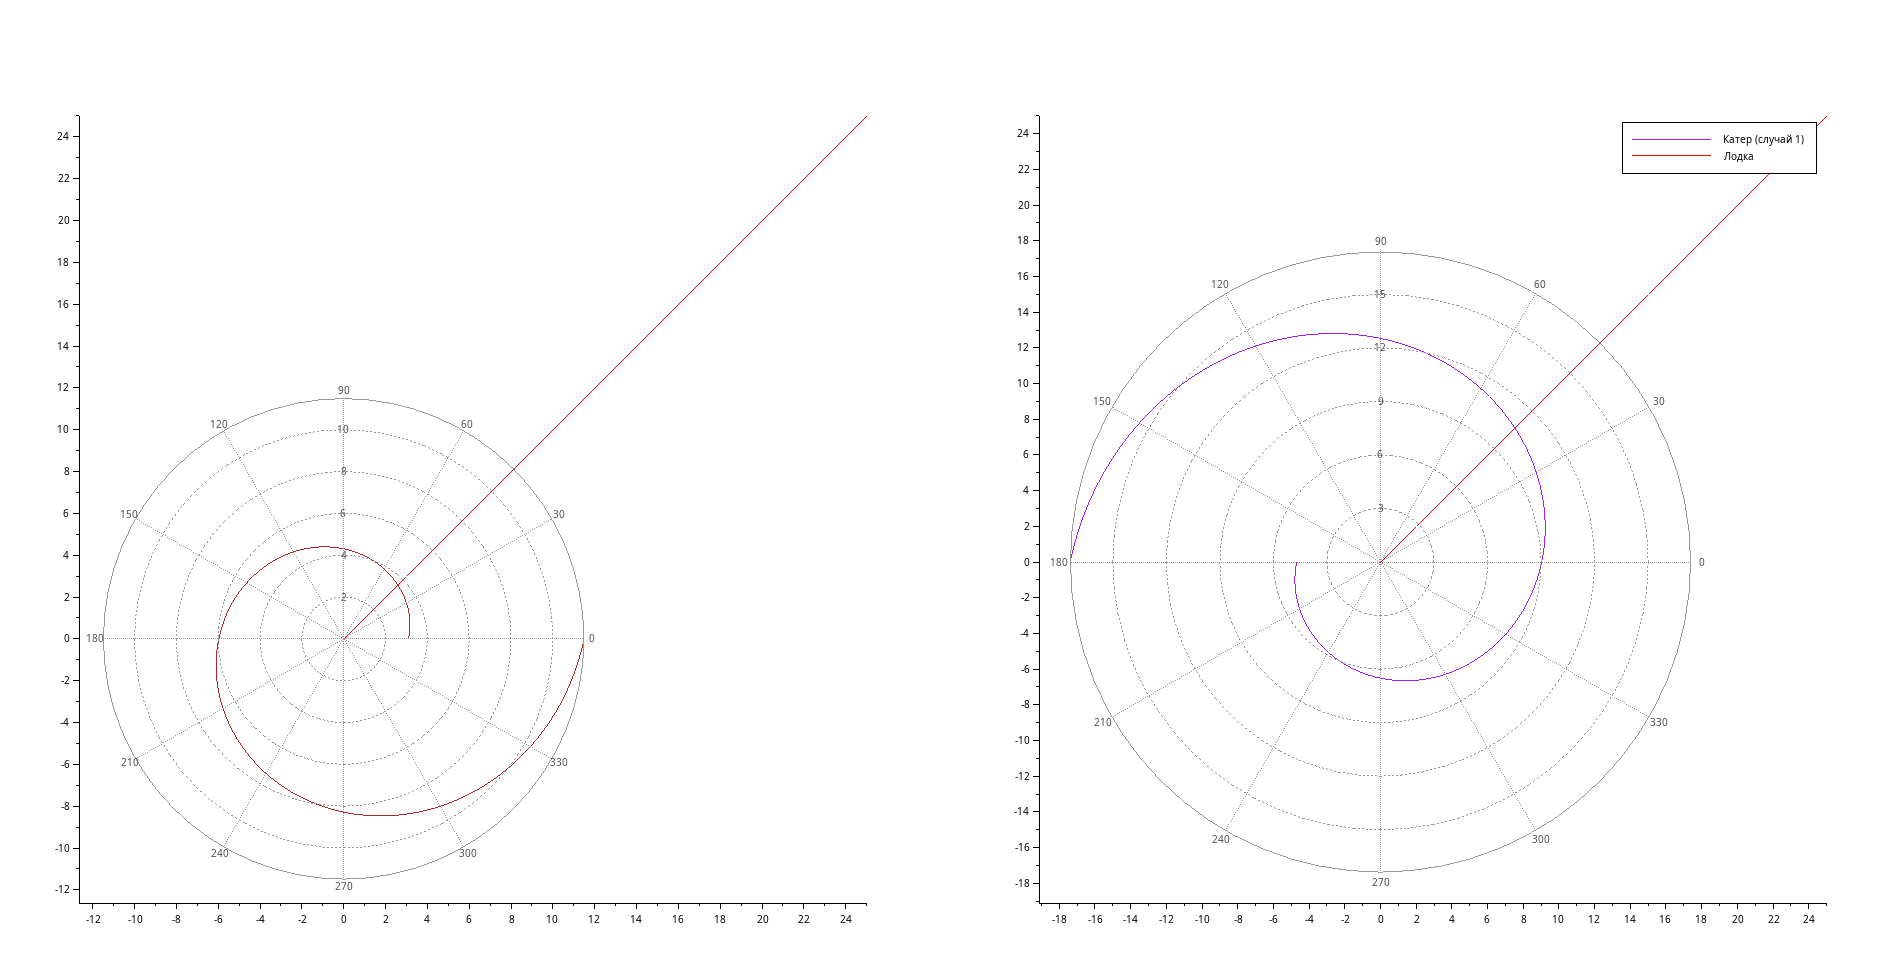
\includegraphics[width=0.7\textwidth,height=\textheight]{image/fig3.png}

}

\caption{\label{fig-001}визуализия с помощью scilab}

\end{figure}%

С точки пересечении(рис.2)

\begin{figure}

\centering{

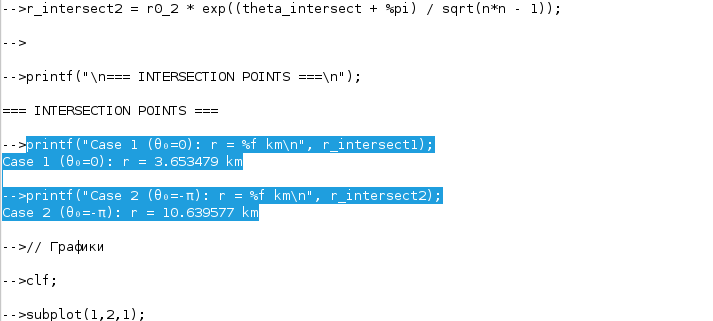
\includegraphics[width=0.7\textwidth,height=\textheight]{image/fig4.png}

}

\caption{\label{fig-001}точки пересечении}

\end{figure}%

Программа scilab

\begin{verbatim}

// Исходные данные
s = 18.3; // начальное расстояние от лодки до катера
n = 4.9; // отношение скоростей катера и лодки
fi = %pi / 4; // угол направления движения лодки
// Функция, описывающая движение катера береговой охраны
function dr = f(theta, r)
dr = r / sqrt(n*n - 1);
endfunction
// Начальные условия для первого случая (катер ближе к полюсу)
r0_1 = s / (n + 1); // x1 = k / (n + 1)
theta0_1 = 0;
theta = 0:0.01:2*%pi;
r1 = ode(r0_1, theta0_1, theta, f);
// Начальные условия для второго случая (катер дальше от полюса)
r0_2 = s / (n - 1); // x2 = k / (n - 1)
theta0_2 = -%pi;
theta2 = -%pi:0.01:%pi;
r2 = ode(r0_2, theta0_2, theta2, f);
// Функция движения лодки браконьеров
function xt = f2(t)
xt = tan(fi) * t;
endfunction
t = 0:1:25;
// Calculate intersection points
theta_intersect = fi;
r_intersect1 = r0_1 * exp(theta_intersect / sqrt(n*n - 1));
r_intersect2 = r0_2 * exp((theta_intersect + %pi) / sqrt(n*n - 1));

printf("Case 1 (θ₀=0): r = %f km\n", r_intersect1);
printf("Case 2 (θ₀=-π): r = %f km\n", r_intersect2);
// Графики
clf;
subplot(1,2,1);
polarplot(theta, r1, style=color('brown')); // катер (случай 1)
plot2d(t, f2(t), style=color('red')); // лодка
subplot(1,2,2);
polarplot(theta2, r2, style=color('purple')); // катер (случай 2)
plot2d(t, f2(t), style=color('red')); // лодка
// Отображение графиков
xtitle("Траектории движения катера и лодки (случай 1 - слева, случай 2 - справа", "�",
legend("Катер (случай 1)", "Лодка", "Катер (случай 2)");
\end{verbatim}

\chapter{Выводы}\label{ux432ux44bux432ux43eux434ux44b}

Выполнив эту работу, я создала математическое моделирование задачи
преследования браконьерской лодки катером береговой охраны и определение
оптимальной траектории движения катера для перехвата цели.


\printbibliography


\end{document}
